\chapter{MAC}

Here, we are using the tri-mode ethernet MAC v0.1.

\begin{enumerate}
\item Introduction

The core of the Tri-mode ethernet MAC is designed from the ground up to be a compact, fast, no-frills core to faciliate streaming data from a widget to a connected computer. For example, the core only supports full-duplex operation in that it does not even look at the CRS (carrier-sense) and COL (collision detection) signals from the PHY (physical layer). And it will generate the ethernet and udp headers so we can simply give it data and it will take care of sending it for us.

\item Features

• Interfaces with the PHY using GMII running 10/100/1000 Mb/s. Support for RGMII is planned.
• Full-duplex support only.
• Raw ethernet frame generation, allowing a pure data input stream.
• Optional UDP/IP packet generation with automatic packetization and framentation of an input data
stream.
• Input and output fifos decoupled from the core logic, so the clock rate of application logic is not tied
to the speed of the ethernet link (barring bandwidth issues).
• Full core uses 288 Spartan 6 logic slices and 2 block RAMs. For comparison, the smallest Spartan 6
has 600 slices and 12 block RAMs. The largest Spartan 6 has 23,038 slices and 268 block RAMs.

\item Interfaces

\begin{itemize}

\item Parameters

\begin{figure}[ht!]
\centering
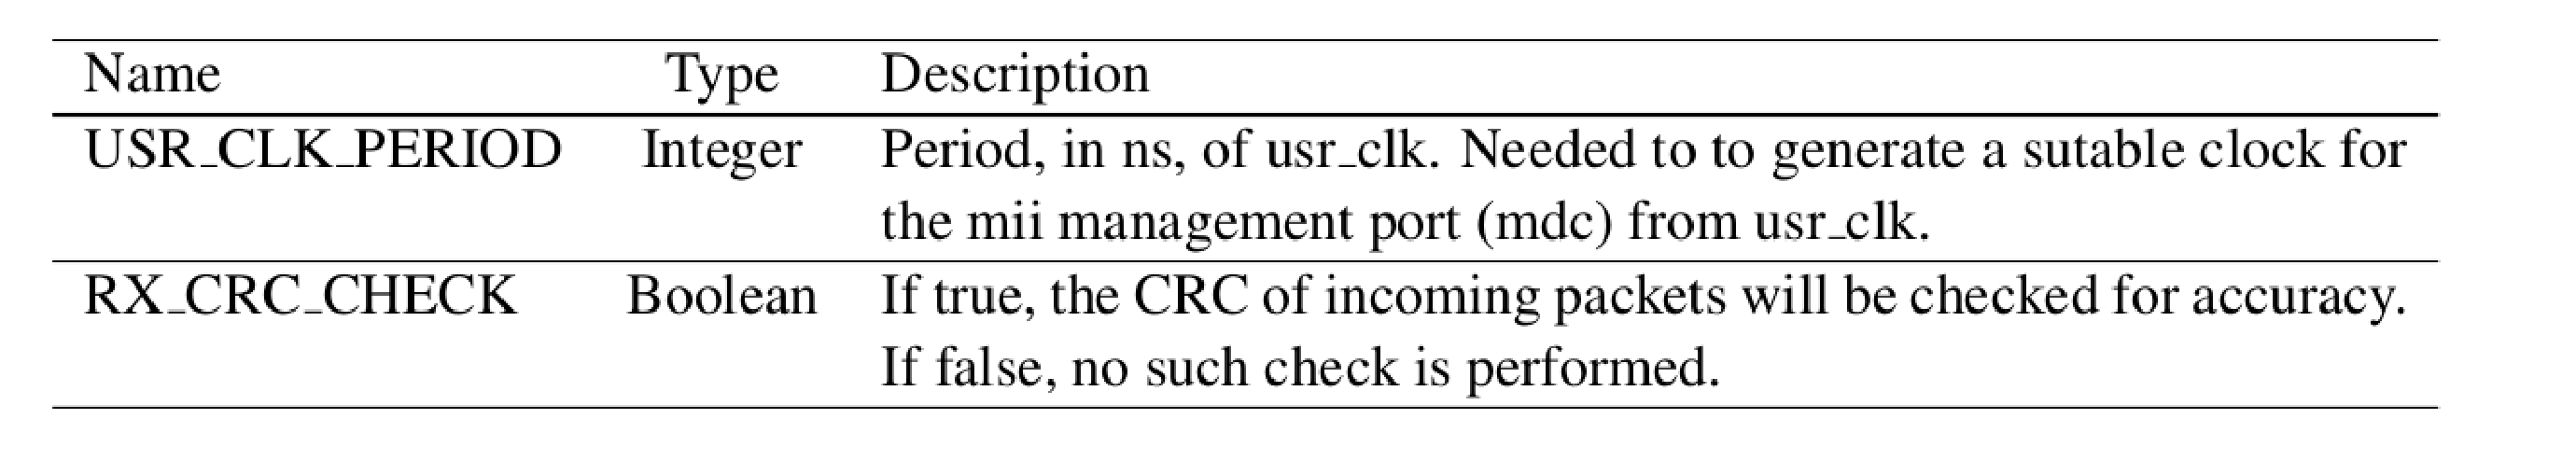
\includegraphics[scale=0.25]{eps/mac1.eps}
\caption{The mac1}
\label{mac1}
\end{figure}

\item Clocks, etc.

\begin{figure}[ht!]
\centering
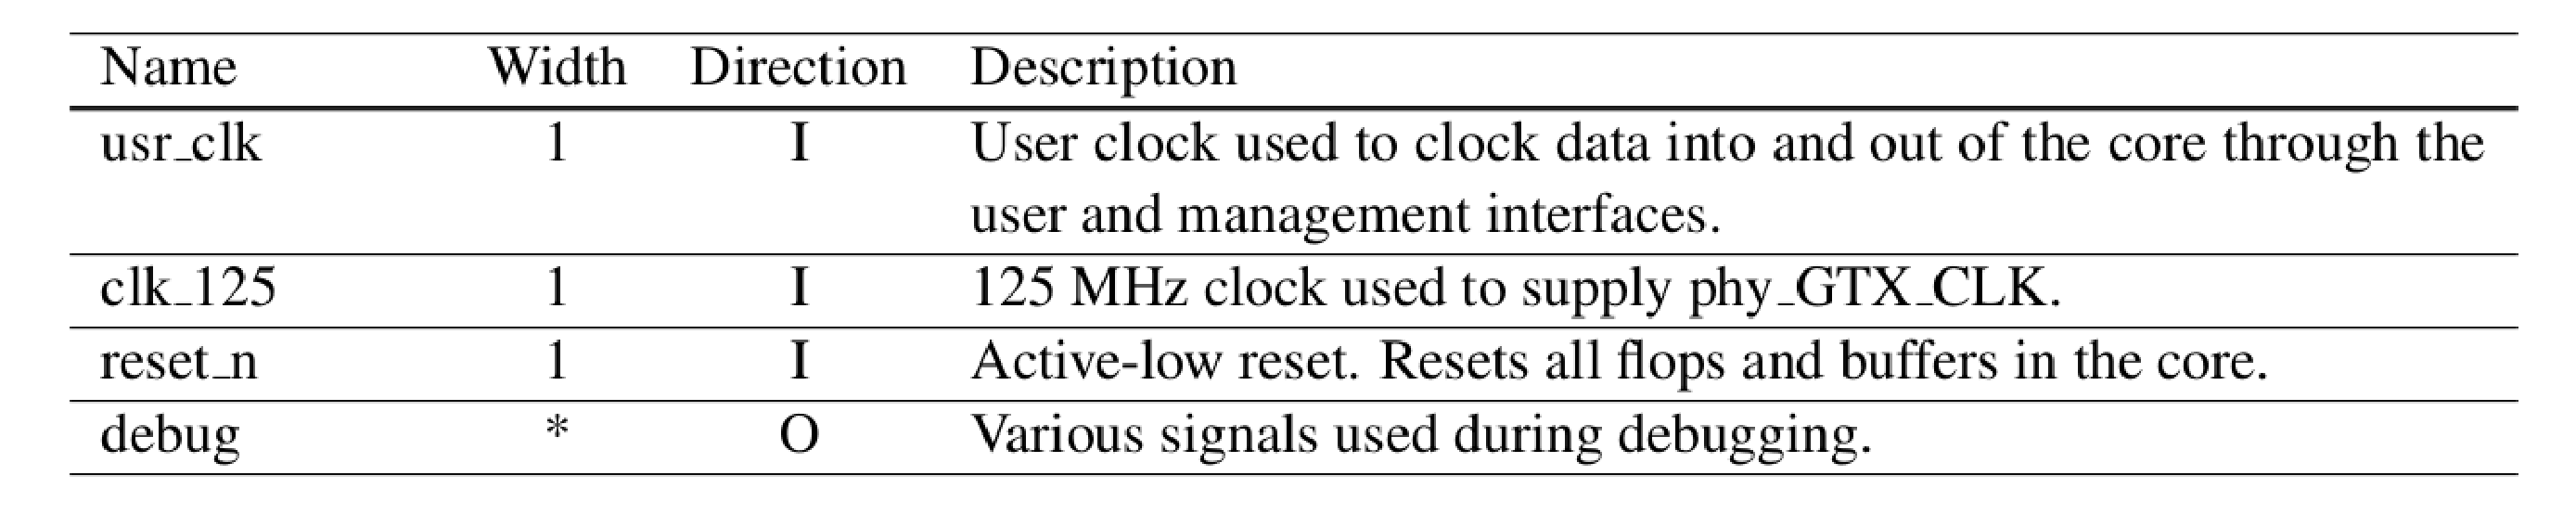
\includegraphics[scale=0.25]{eps/mac2.eps}
\caption{mac2}
\label{mac2}
\end{figure}

\end{itemize}

\item Configuration

Instead of implementing internal registers to indicate the source and destination MAC address, these values are simply ports into the core. 

\begin{figure}[ht!]
\centering
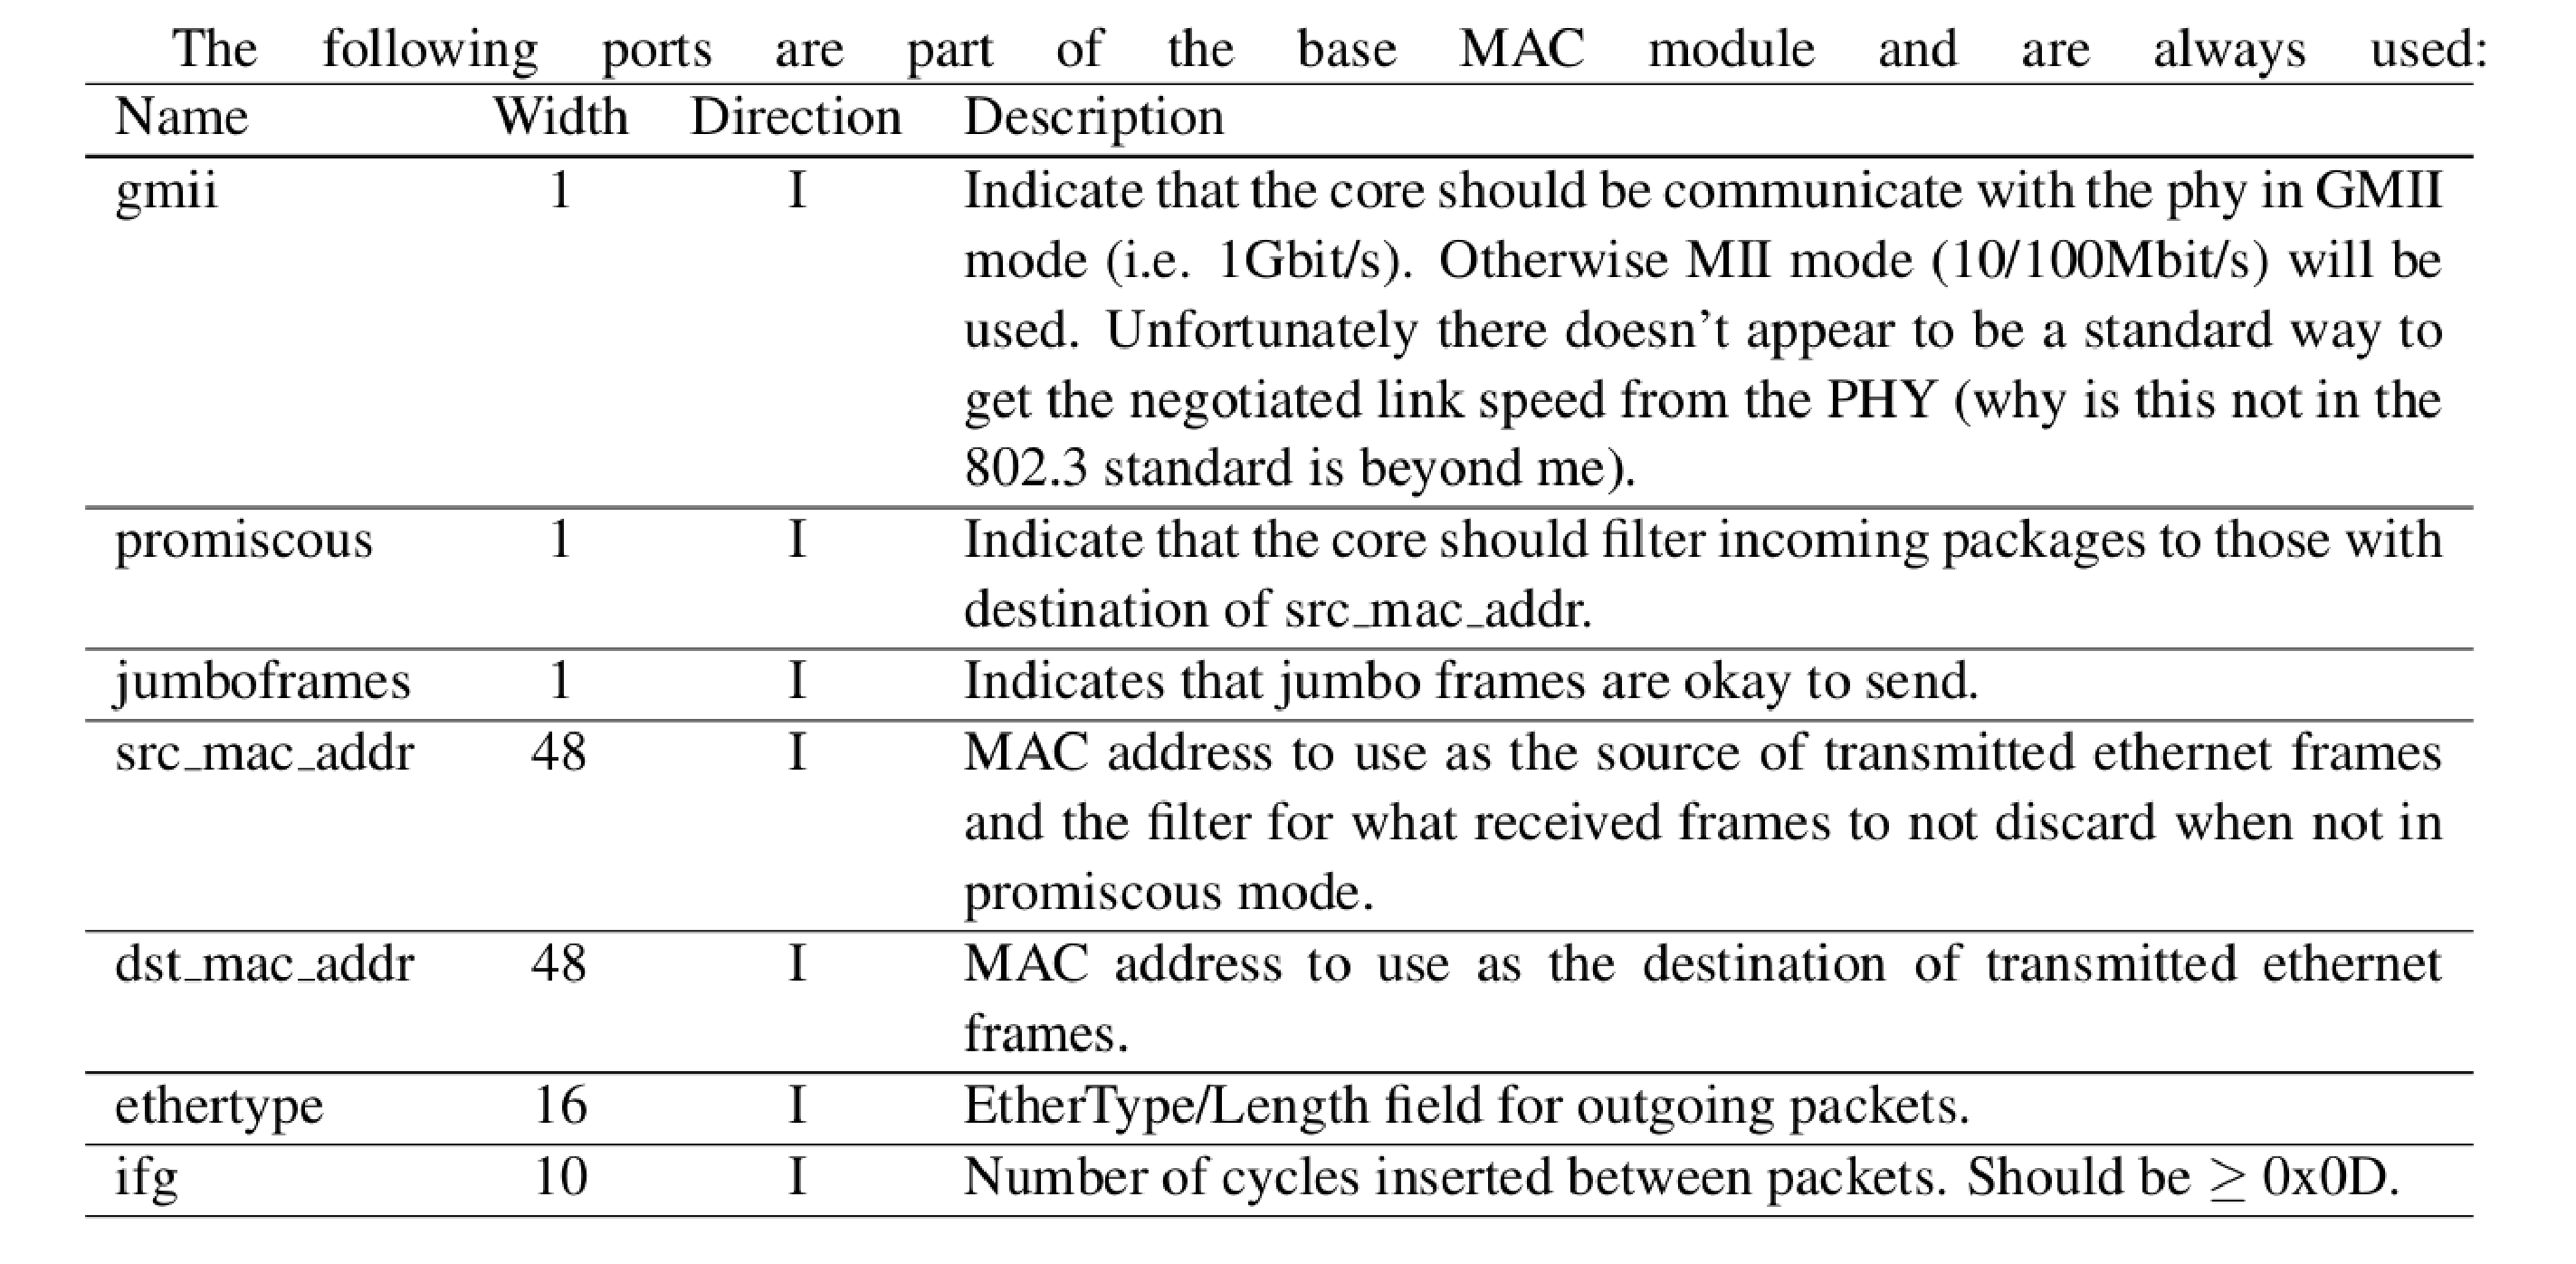
\includegraphics[scale=0.25]{eps/mac3.eps}
\caption{mac3}
\label{mac3}
\end{figure}

\begin{figure}[ht!]
\centering
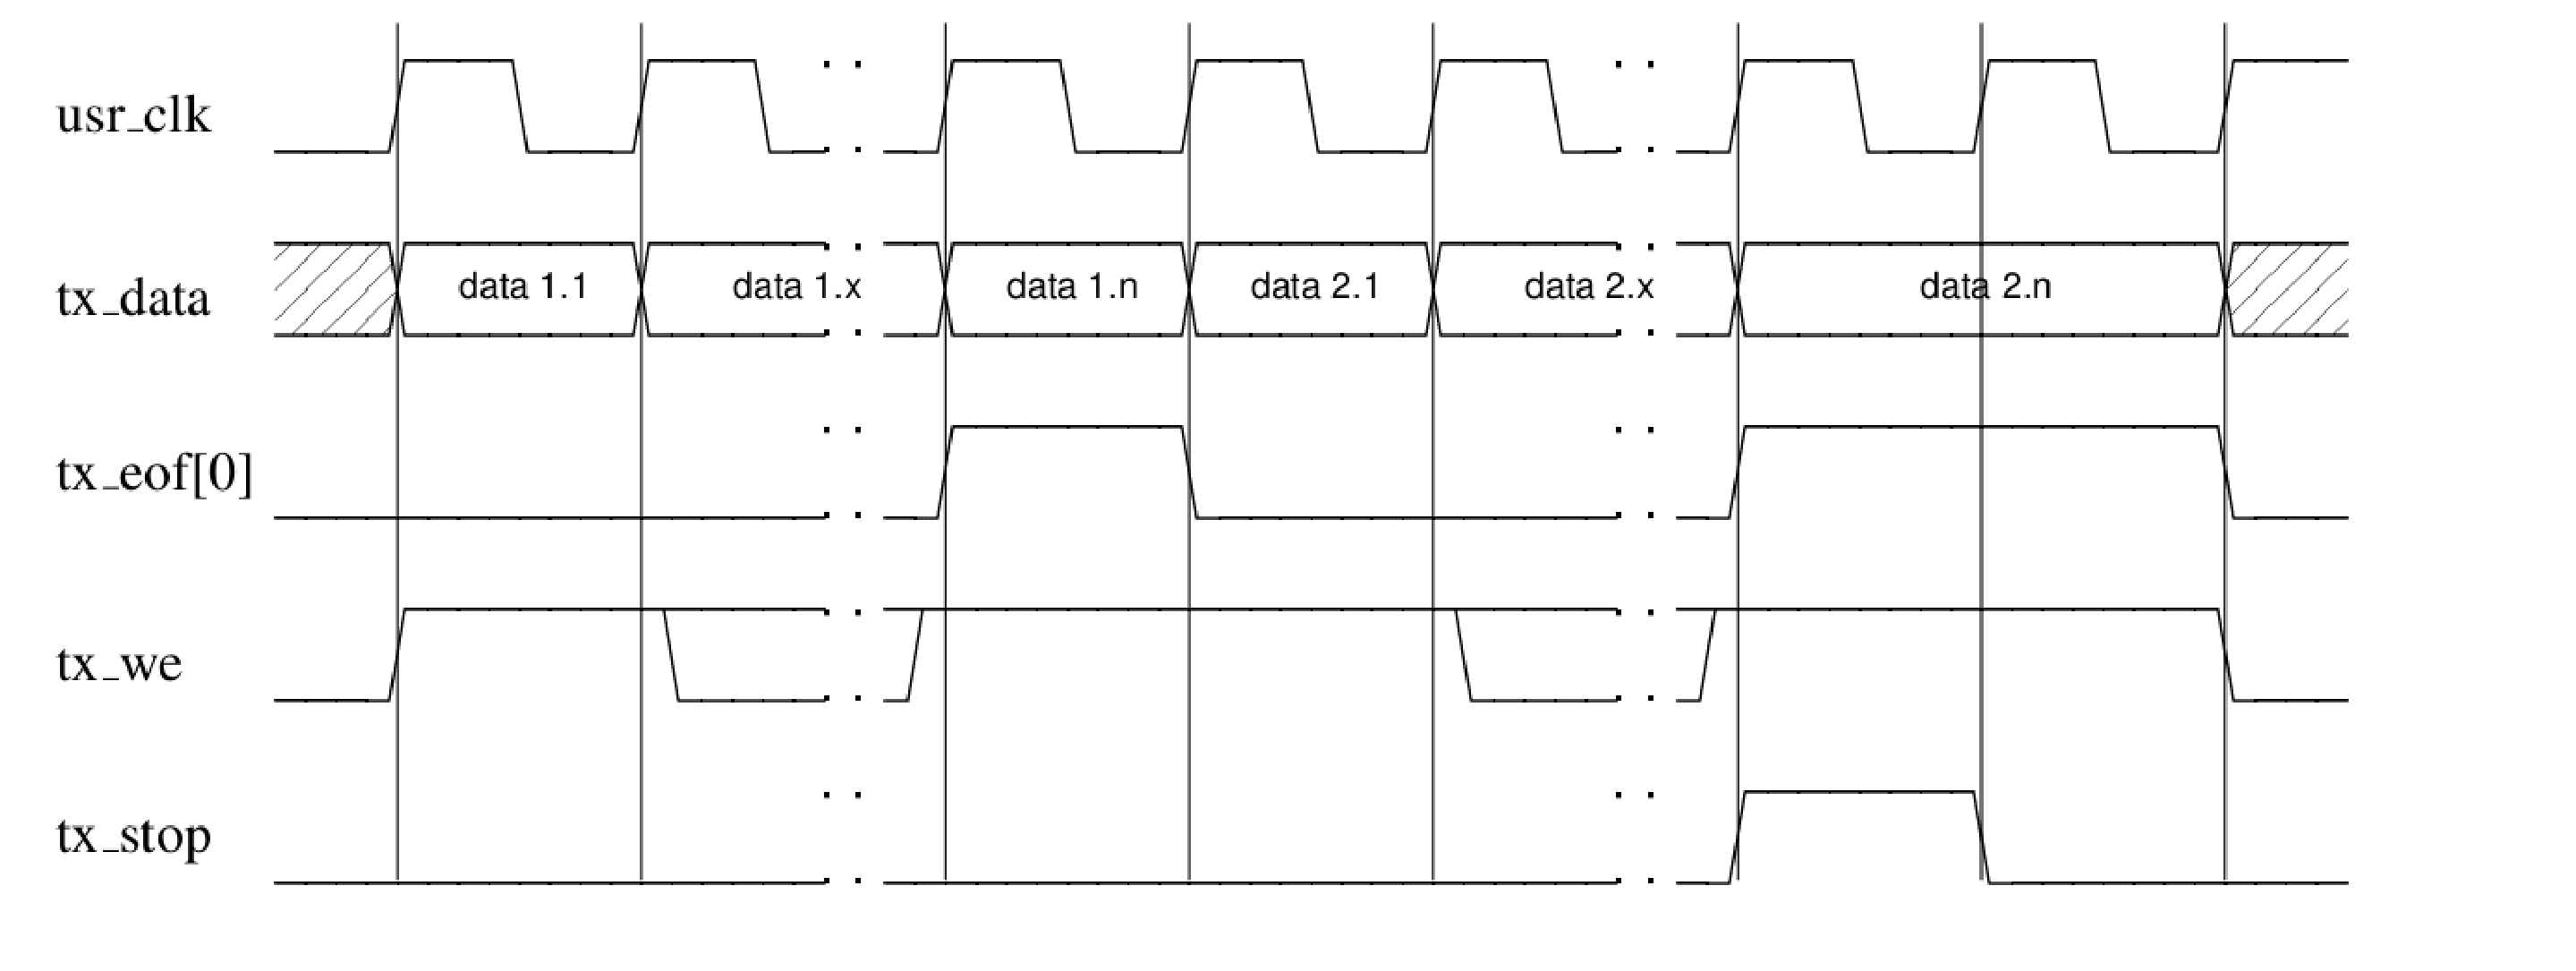
\includegraphics[scale=0.25]{eps/mac4.eps}
\caption{mac4}
\label{mac4}
\end{figure}

In Figure~\ref{mac4}, we can see the timing diagram of two back to back 32-bit aligned packet transmissions, with the final word of the second packet being interrupted by a full input fifo.

\item Transmission

The interface used to send packets/frames is a standard FIFO write interface with addition of an end-of-frame port (tx eo f ) that is used to split incoming data into frames.

\begin{figure}[ht!]
\centering
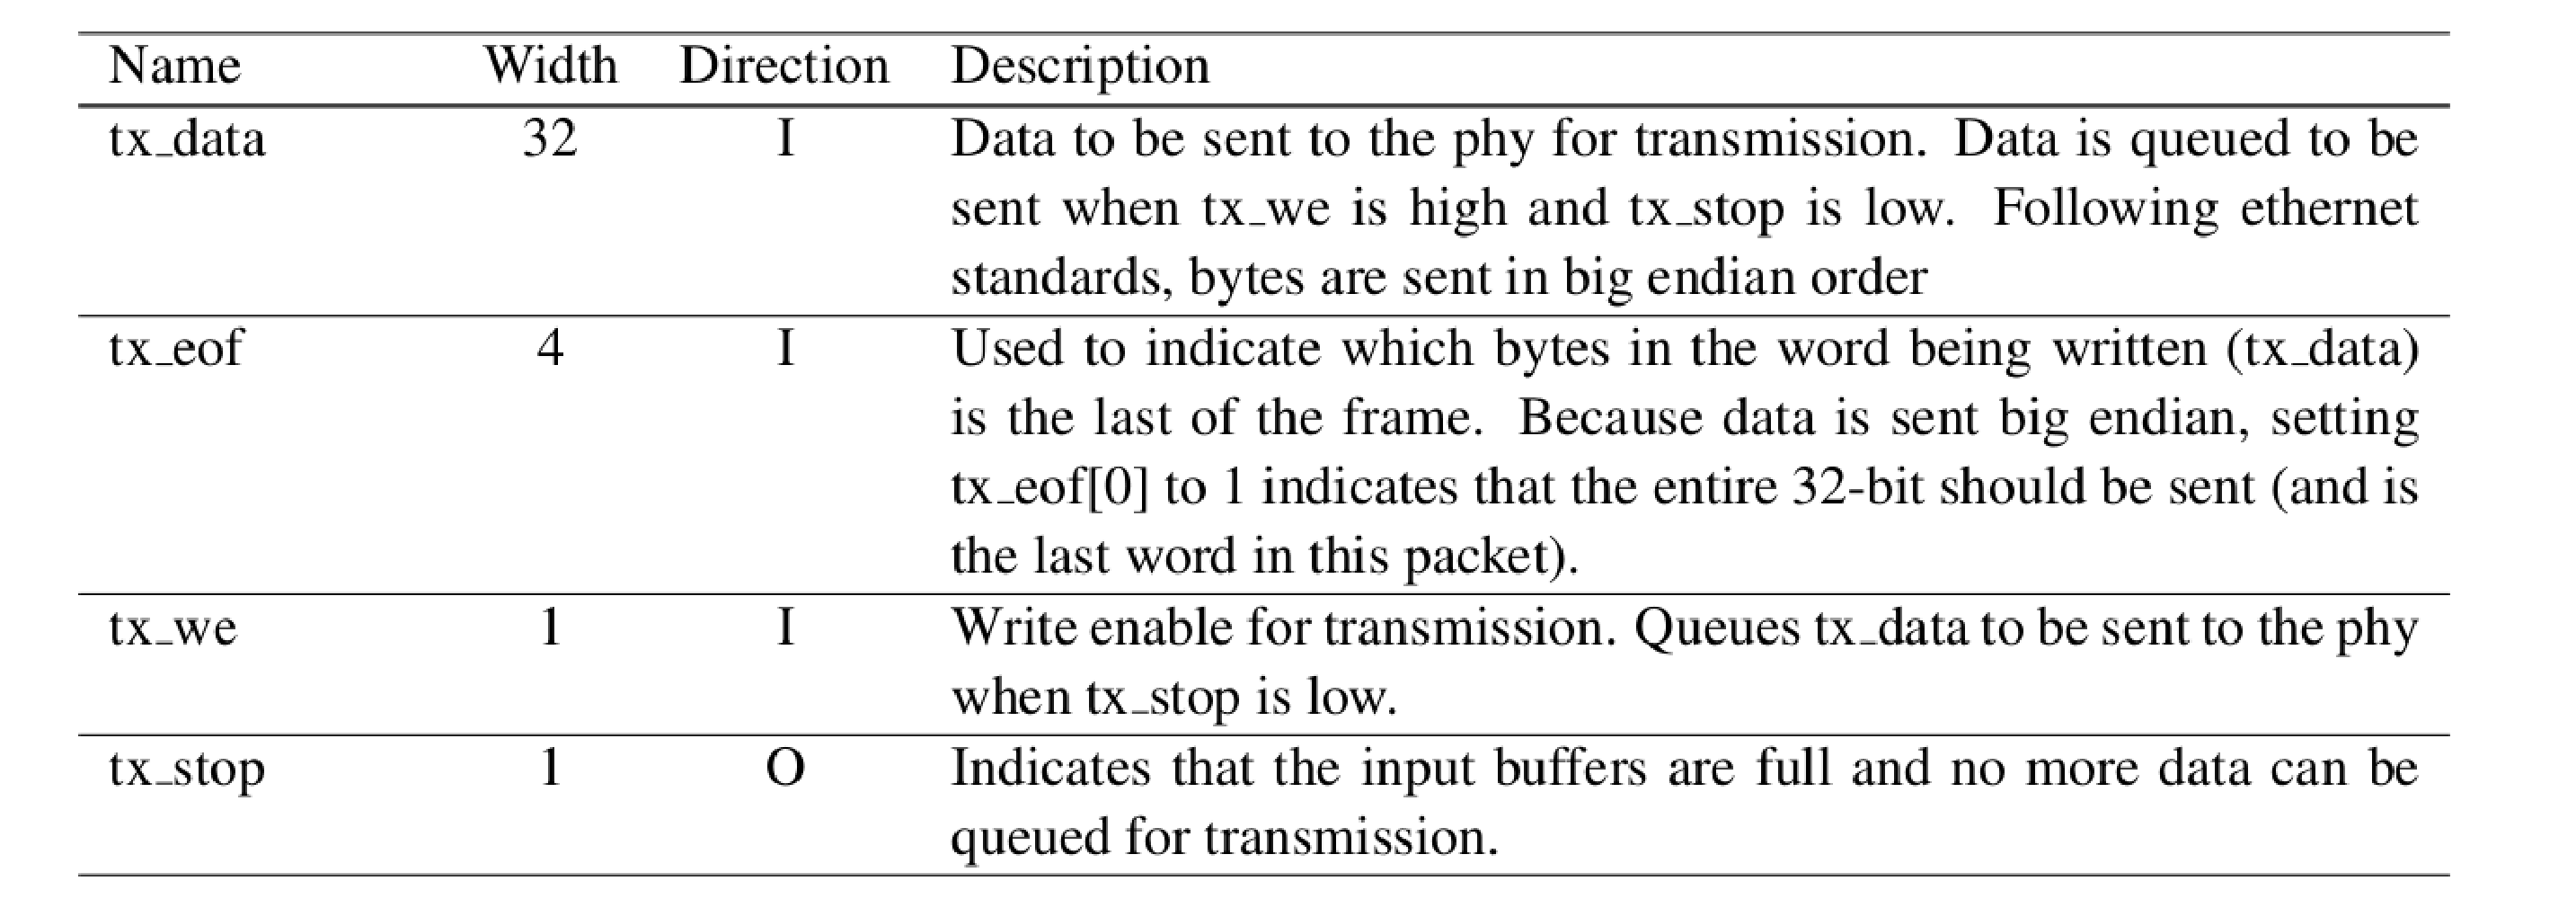
\includegraphics[scale=0.25]{eps/mac5.eps}
\caption{mac5}
\label{mac5}
\end{figure}


If the input fifo runs out of data while the MAC is sending a packet, an error condition will be raised and the packet will not be sent. Operating at 1Gbps, the PHY will transmit approximately 100MB/s from the input fifo. Therefore, if data word is supplied every clock, the user clock must be at least 25 MHz, an easy target for most FPGAs. Alternatively, if the user clock is faster, data need not be supplied on each clock. For example, a 100 MHz user clock means that once data is first written to the input fifo, the rest of the data can come at a rate as slow as one word every 4 clocks.


\item Reception

The interface used to receive packets is a standard FIFO read interface, with the addition of an end-of-frame port (rx eo f ).

\begin{figure}[ht!]
\centering
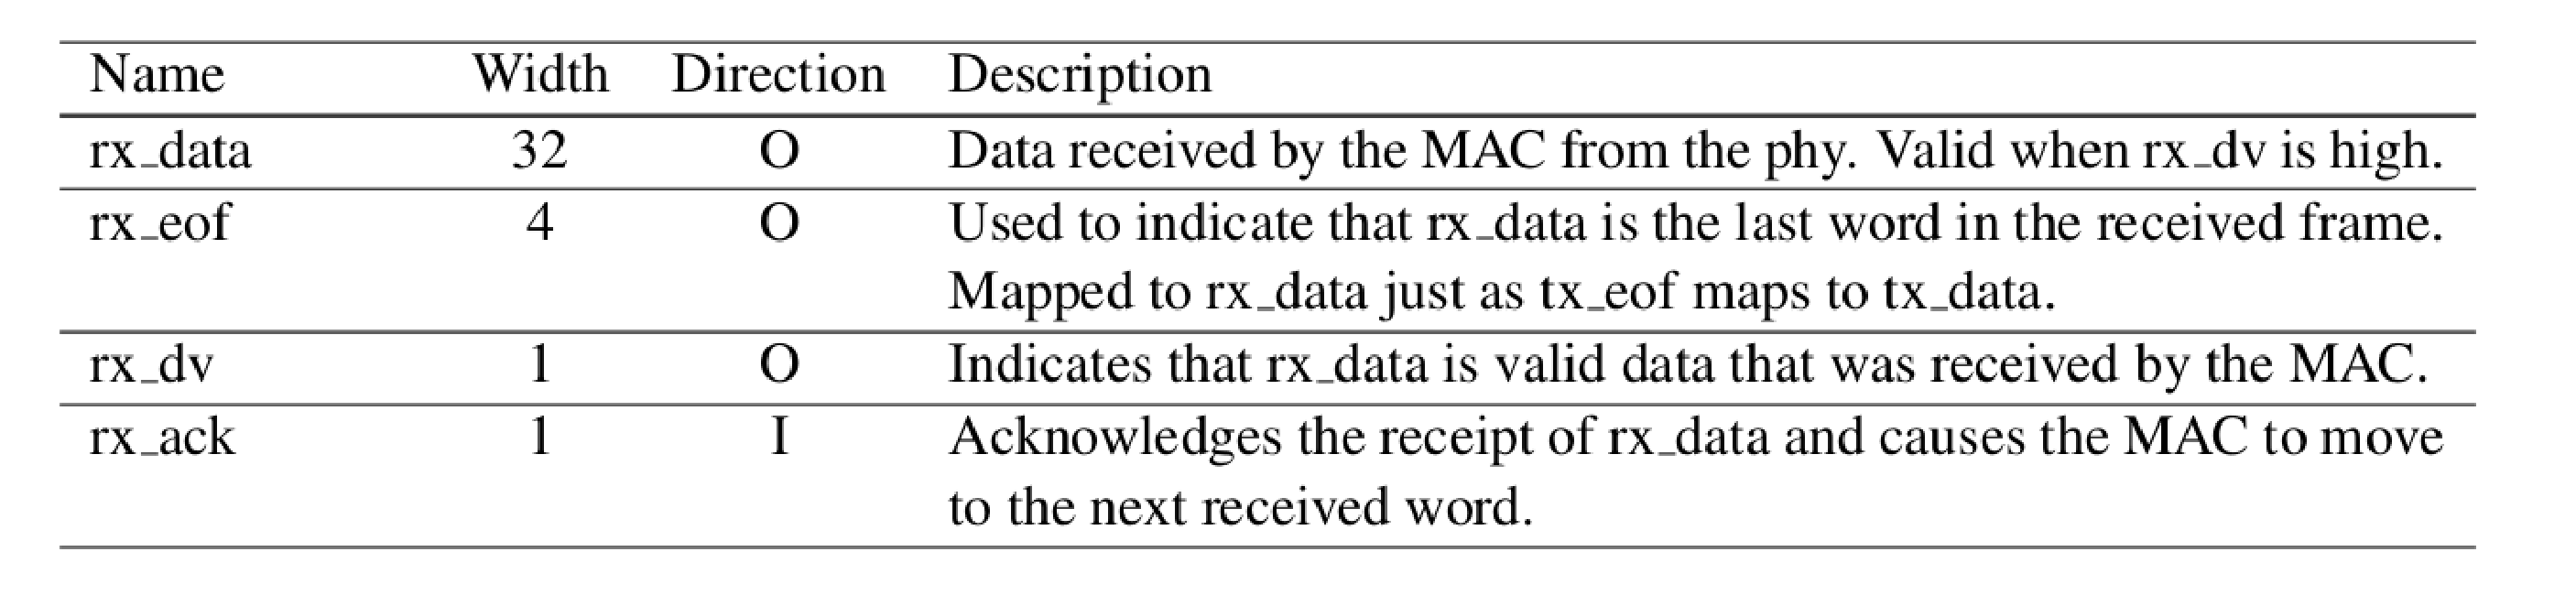
\includegraphics[scale=0.25]{eps/mac6.eps}
\caption{mac6}
\label{mac6}
\end{figure}

\item Management

The following ports are used to read and write the MII management registers on the PHY. If they are left unconnected, the MII management module will be optimized away by the synthesis tools.

\begin{figure}[ht!]
\centering
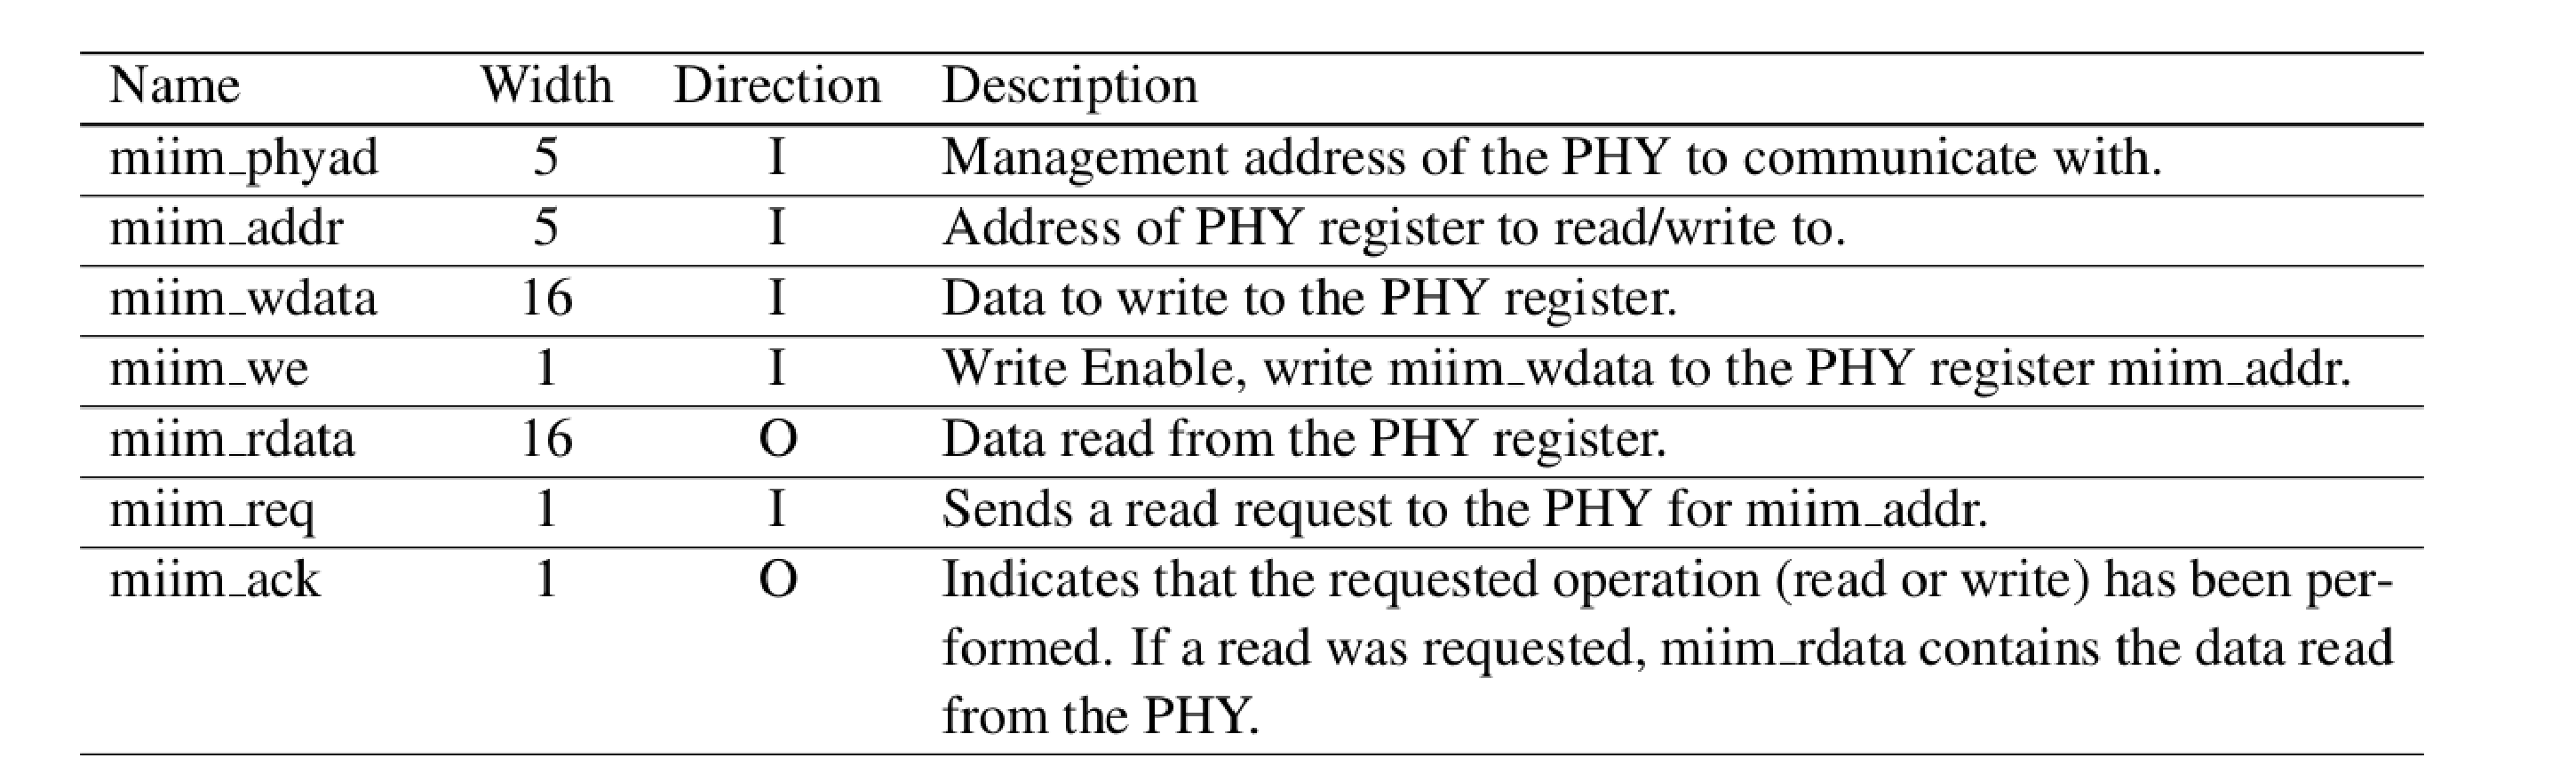
\includegraphics[scale=0.25]{eps/mac7.eps}
\caption{mac7}
\label{mac7}
\end{figure}

\item UDP/IP

When the UDP/IP Wrapper is used, the ethertype port is removed and the following configuration ports are added.

\begin{figure}[ht!]
\centering
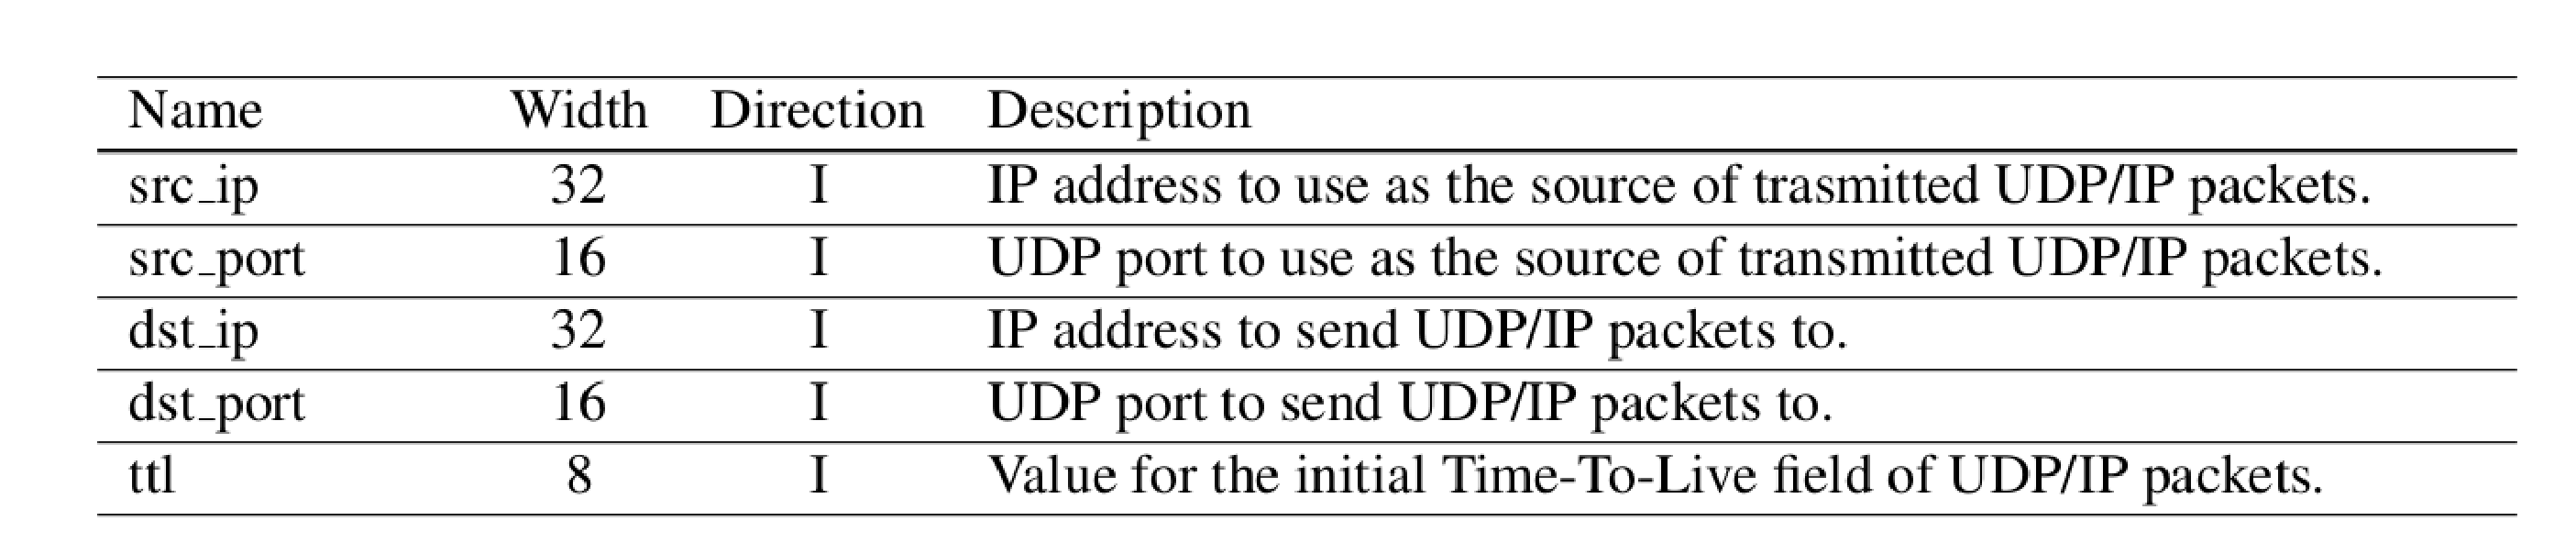
\includegraphics[scale=0.25]{eps/mac8.eps}
\caption{mac8}
\label{mac8}
\end{figure}


\item PHY

The PHY ports are the standard GMII ports that should be tied directly to pins connected to an ethernet PHY.

\begin{figure}[ht!]
\centering
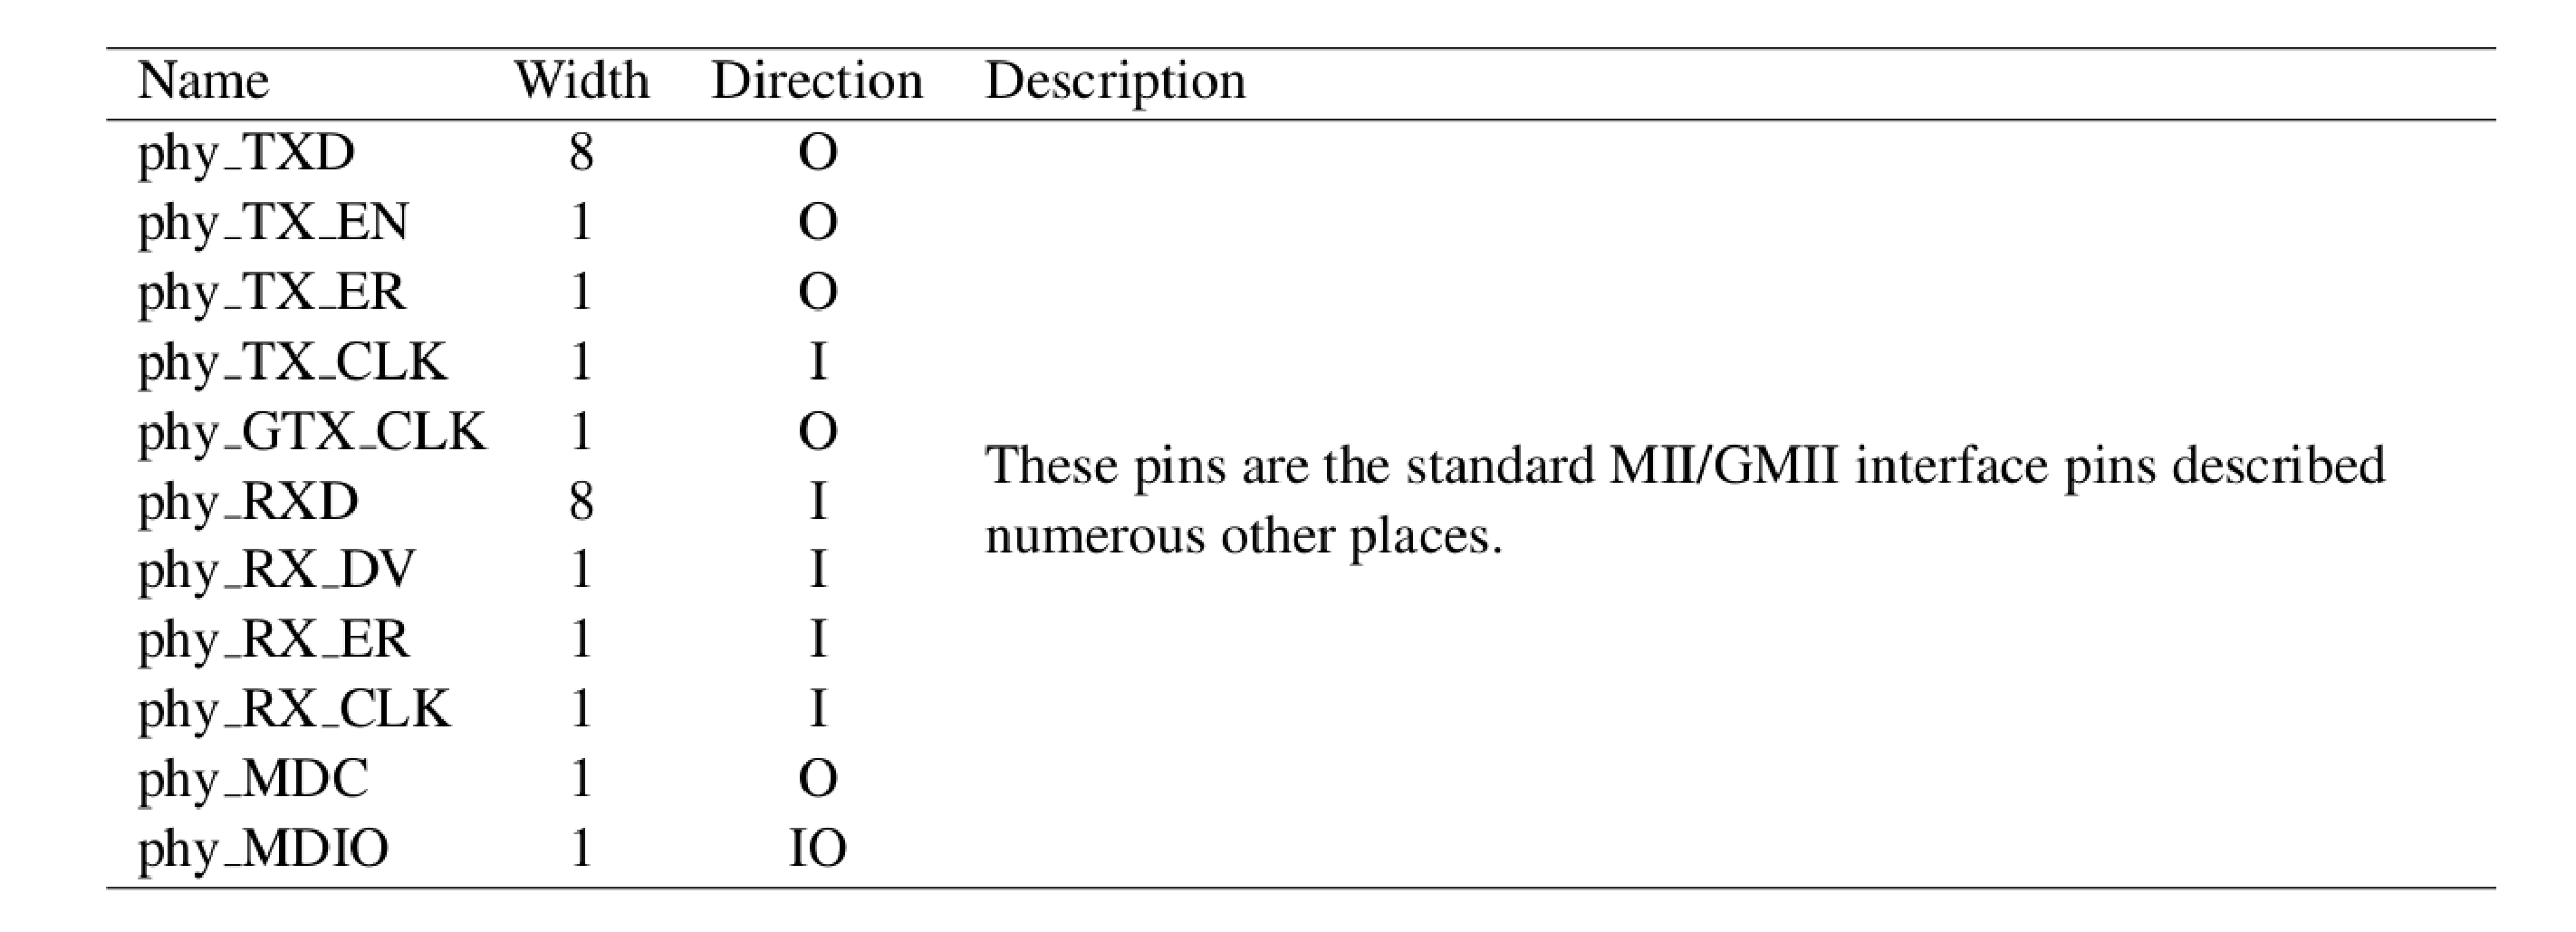
\includegraphics[scale=0.25]{eps/mac9.eps}
\caption{mac9}
\label{mac9}
\end{figure}

\item Reconciliation

The reconcilation modules provides a common interface to the rest of the core regardless of the speed of the ethernet link. This is done by providing internal clocks to both the tx (int tx clk) and rx (int rx clk) modules which can be used to send data to the reconciliation layer eight bits a clock.

If gmii is high we are operating at gigabit speeds and the phy sends and receives a full eight bits of data each 8ns. For transmission, clk 125 is used as both int tx clk and sent as phy GTXCLK, synchronizing all tranmission to that one 125 MHz clock. Likewise, all reception is synchronized to the 125 MHz phy RXCLK, which is sent as int rx clk.

If gmii is low we are operating at 10 or 100 Mbits per second and only four bits of the databus to the phy is used. For transmission, the phy expects four bits every cycle of the phy supplied phy TXCLK; to maintain an eight bit interface with the rest of the mac, phy TXCLK is divided in half and sent as int tx clk. Likewise, the phy sends four bits every phy RXCLK, so this is divided in half and sent as int rx clk.


\item Architecture

The MAC core is split up into three main components: tranmission, reception, and reconciliation. The transmission blocks, txfifo, tx engine, and crc gen, are responsible for taking user data and sending it to the reconcilia- tion module, which sends it to the ethernet phy. Likewise the recption blocks, rx usr if, rx pkt fifo, rxfifo, rx engine, and crc chk, are responsible for taking data from the reconciliation layer, throwing away bad frames, and presenting it to the user. The reconciliation layer handles with the GMII interface to the phy and deals with differences between 10/100Mbit operation and gigabit operation.

\begin{figure}[ht!]
\centering
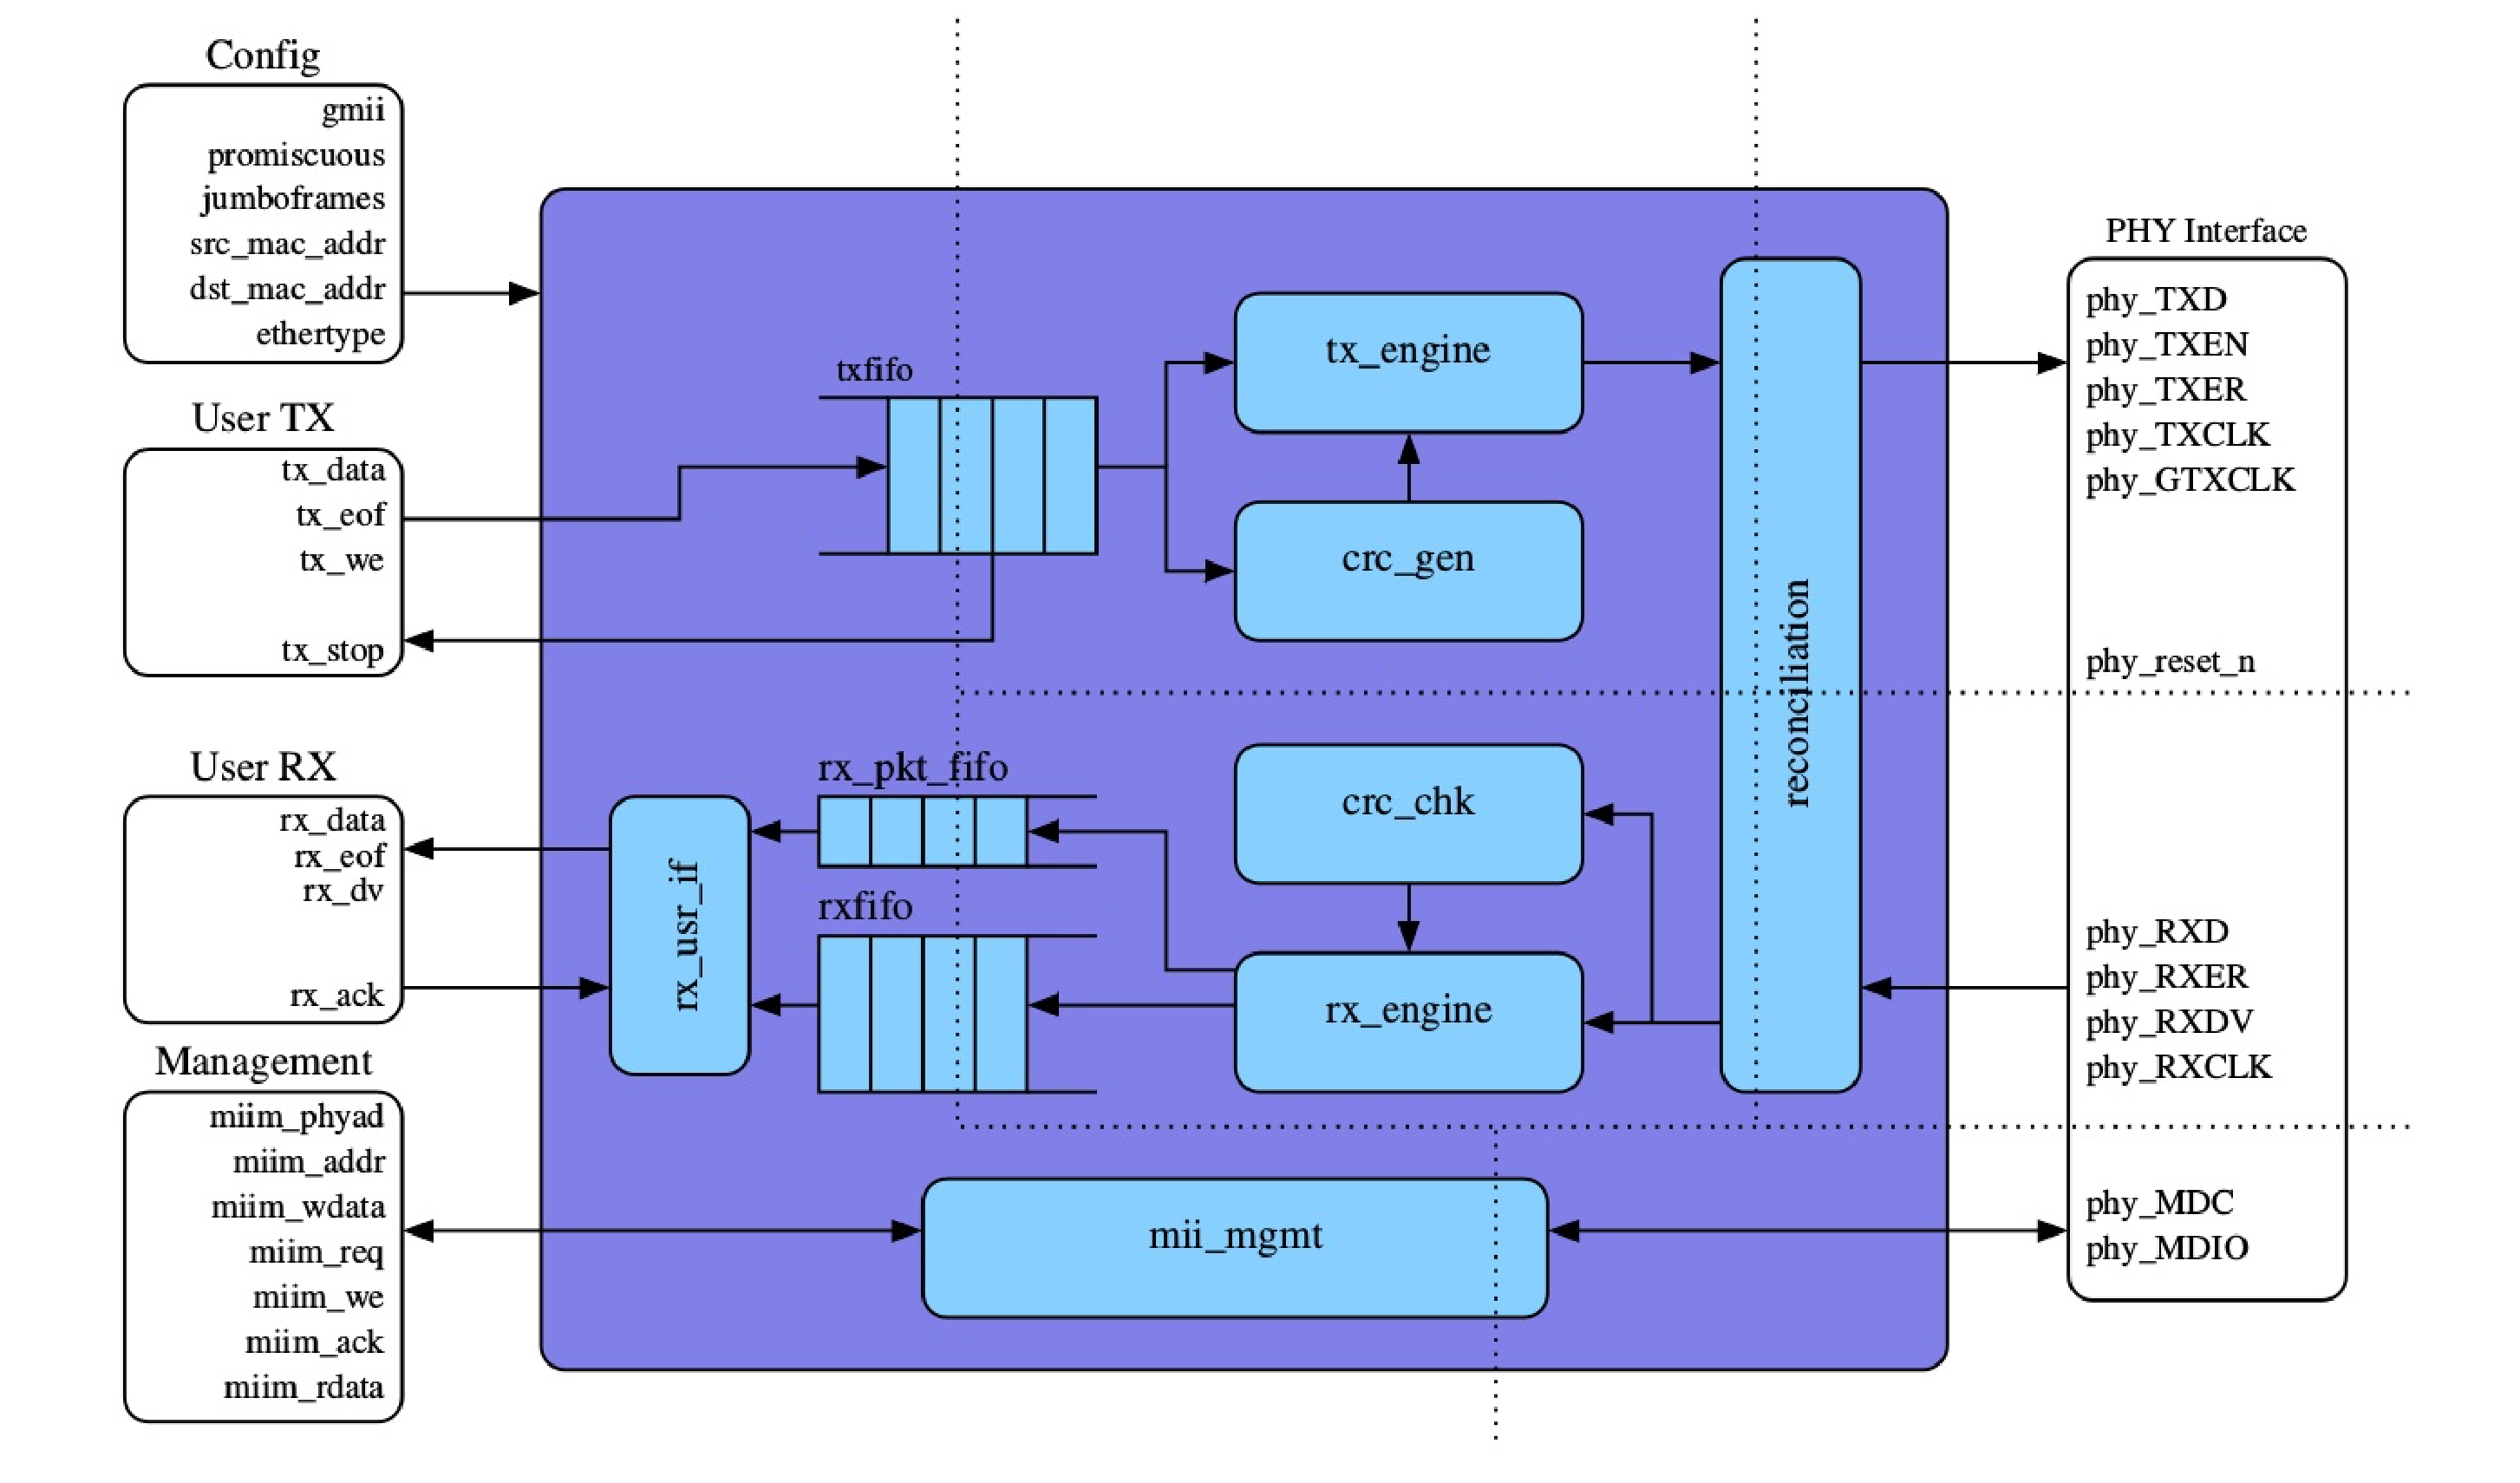
\includegraphics[scale=0.25]{eps/mac10.eps}
\caption{mac10}
\label{mac10}
\end{figure}

\end{enumerate}

